To solve the initial problem it was created a small app that takes an image from the test dataset and print its label. After that the model predicts the value of the particular image and prints the comparison between the true label and the predicted one. This app can easily be expanded further in a next stage of development to take as input new histopathology images. 
The test image:
\begin{figure}[H]
    \centering
    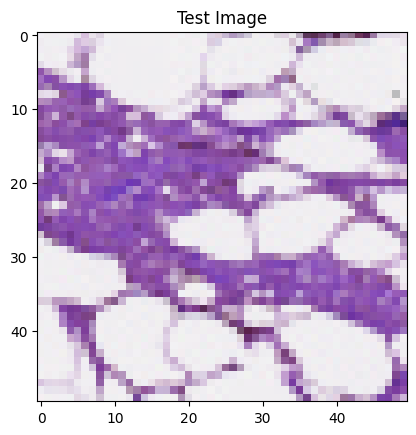
\includegraphics[width=0.6\textwidth]{Images/test_image.png}
    \caption{Test Image}
    \label{fig:example}
\end{figure}
The particular results for the image above:
\begin{figure}[H]
    \centering
    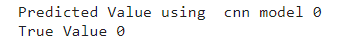
\includegraphics[width=0.6\textwidth]{Images/results.png}
    \caption{Results}
    \label{fig:example}
\end{figure}